\documentclass[10pt]{article}

\usepackage[a4paper,margin=0.65in]{geometry}
\usepackage{amsmath,amssymb}
\usepackage{graphicx}
\usepackage{booktabs}
\usepackage{array}
\usepackage{float}
\usepackage{hyperref}
\usepackage{enumitem}
\usepackage{xcolor}
\usepackage{tikz}
\usetikzlibrary{positioning,arrows.meta,shapes.geometric}

\setlist{nosep,leftmargin=*}
\renewcommand{\arraystretch}{1.2}
\setlength{\parindent}{0pt}
\setlength{\parskip}{2pt}

\tikzset{
layer/.style={
draw,
rounded corners,
minimum width=1.5cm,
minimum height=0.6cm,
align=center,
fill=blue!10,
font=\scriptsize
},
arrow/.style={
-{Latex[length=2mm]},
thin
}
}

\begin{document}

%%%%%%%%%%%%%%%%%%%%%%%%%%%%%%%%%%%%%%%%%%%%%%%%%%%%%%%%%%%%
% TITLE
%%%%%%%%%%%%%%%%%%%%%%%%%%%%%%%%%%%%%%%%%%%%%%%%%%%%%%%%%%%%

\begin{center}

{\large\textbf{Shiv Nadar University Chennai}}

\vspace{2mm}

{\normalsize\textbf{CS3807 -- Deep Learning Laboratory}}

\vspace{2mm}

{\large\textbf{Experiment 5}}

\vspace{1mm}

{\normalsize\textbf{Comprehensive Study of CNN Training, Regularization,}}

{\normalsize\textbf{Optimization, Hyperparameter Tuning, Transfer Learning}}

{\normalsize\textbf{and Cross-Validation}}

\end{center}

\vspace{3mm}

\begin{tabular}{|p{3.4cm}|p{9.0cm}|p{1.4cm}|}
\hline
Degree \& Branch &
B.Tech Artificial Intelligence \& Data Science &
Semester V\\
\hline
Subject Code \& Name &
CS3807 -- Deep Learning Laboratory &
AY: 2026--27\\
\hline
\end{tabular}

%%%%%%%%%%%%%%%%%%%%%%%%%%%%%%%%%%%%%%%%%%%%%%%%%%%%%%%%%%%%
\section*{1. Objective}

The objective of this experiment is to systematically study the effect of
weight initialization, regularization, optimization algorithms, CNN
hyperparameters, transfer learning, fine-tuning and cross-validation on
image classification performance.

The experiment uses a single CNN architecture, MobileNetV2, and the
Oxford-IIIT Pet dataset. Students will analyze the effect of individual
design choices using training/validation curves and finally select a
suitable configuration using 5-fold cross-validation.

%%%%%%%%%%%%%%%%%%%%%%%%%%%%%%%%%%%%%%%%%%%%%%%%%%%%%%%%%%%%
\section*{2. Learning Outcomes}

After completing this experiment, students will be able to:

\begin{itemize}
\item explain different weight initialization strategies;
\item identify and analyze overfitting using training and validation curves;
\item compare SGD, Momentum, RMSProp and Adam;
\item explain CNN hyperparameters such as kernel size, stride, padding and pooling;
\item understand Batch Normalization and Dropout;
\item perform transfer learning and fine-tuning using MobileNetV2;
\item tune important training hyperparameters;
\item apply 5-fold cross-validation for model selection; and
\item justify the final model using accuracy, variability and computational cost.
\end{itemize}

%%%%%%%%%%%%%%%%%%%%%%%%%%%%%%%%%%%%%%%%%%%%%%%%%%%%%%%%%%%%
\section*{3. Dataset and Experimental Setup}

\textbf{Dataset: Oxford-IIIT Pet Dataset}

The Oxford-IIIT Pet Dataset contains images of cats and dogs belonging
to 37 breeds. The images are RGB and have different spatial dimensions.
For this experiment, all images are resized to

\[
224\times224\times3.
\]

The dataset is suitable for demonstrating transfer learning using
ImageNet-pretrained CNNs.

\textbf{Experimental considerations:}

\begin{itemize}
\item Use RGB images resized to $224\times224$.
\item Normalize the input images according to the pretrained model requirements.
\item Maintain separate training, validation and test data.
\item The test set must remain untouched during hyperparameter selection.
\item Use MobileNetV2 because it is computationally lighter than many
large CNN architectures and is more suitable for CPU-based laboratory work.
\end{itemize}

%%%%%%%%%%%%%%%%%%%%%%%%%%%%%%%%%%%%%%%%%%%%%%%%%%%%%%%%%%%%
\section*{4. MobileNetV2 Architecture}

MobileNetV2 is a lightweight CNN architecture designed to reduce
computational complexity while maintaining good image representation.

Its important components include:

\begin{itemize}
\item depthwise convolution;
\item pointwise $1\times1$ convolution;
\item inverted residual blocks;
\item linear bottlenecks;
\item batch normalization; and
\item ReLU6 activation.
\end{itemize}

A simplified representation is:

\begin{center}
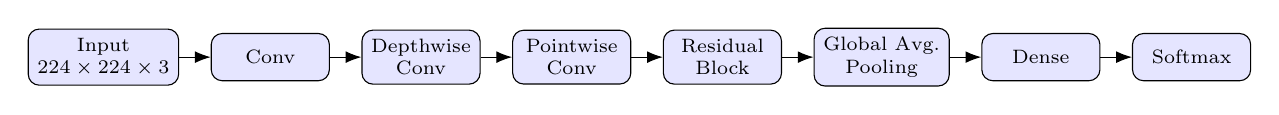
\begin{tikzpicture}[node distance=4mm]

\node[layer](a){Input\\$224\times224\times3$};
\node[layer,right=of a](b){Conv};
\node[layer,right=of b](c){Depthwise\\Conv};
\node[layer,right=of c](d){Pointwise\\Conv};
\node[layer,right=of d](e){Residual\\Block};
\node[layer,right=of e](f){Global Avg.\\Pooling};
\node[layer,right=of f](g){Dense};
\node[layer,right=of g](h){Softmax};

\foreach \x/\y in {a/b,b/c,c/d,d/e,e/f,f/g,g/h}
\draw[arrow](\x)--(\y);

\end{tikzpicture}
\end{center}

\textbf{Note:} The above diagram is a simplified conceptual representation
rather than the complete MobileNetV2 architecture.

%%%%%%%%%%%%%%%%%%%%%%%%%%%%%%%%%%%%%%%%%%%%%%%%%%%%%%%%%%%%
\section*{5. Weight Initialization}

Weight initialization determines the initial values of trainable weights
before training begins. A suitable initialization can improve convergence
and reduce problems such as vanishing or exploding activations.

Students should investigate:

\begin{itemize}
\item Zero initialization
\item Random initialization
\item Xavier/Glorot initialization
\item He initialization
\end{itemize}

\subsection*{Expected Analysis}

Students should compare the initialization strategies using:

\textbf{Plot 1: Training Loss vs. Epoch}

\begin{itemize}
\item X-axis: Epoch
\item Y-axis: Training Loss
\item Plot one curve for each initialization method.
\end{itemize}

\begin{figure}[H]
\centering
\includegraphics[width=0.8\linewidth]{Plot1_TrainLoss_Init.eps}
\label{fig:TrainLoss}
\end{figure}
The plot shows training loss for different initialization methods. Zero initialization hardly learns, while random, Xavier and He reduce the loss rapidly. Proper initialization helps gradients flow and allows the network to learn effectively.
\vspace{0.5cm}

\textbf{Plot 2: Validation Accuracy vs. Epoch}

\begin{itemize}
\item X-axis: Epoch
\item Y-axis: Validation Accuracy (\%)
\item Plot one curve for each initialization method.
\end{itemize}

\begin{figure}[H]
\centering
\includegraphics[width=0.8\linewidth]{Plot2_ValAcc_Init.eps}
\label{fig:ValidationAccuracy}
\end{figure}
Validation accuracy remains almost zero for zero initialization, while the other methods quickly reach around 80–90 percent. This happens because zero initialization makes neurons learn identical features, whereas proper initialization breaks this symmetry.
Xavier initialization gives faster and more stable convergence.

\vspace{0.5cm}

% Students should identify which initialization gives faster and more
% stable convergence.

%%%%%%%%%%%%%%%%%%%%%%%%%%%%%%%%%%%%%%%%%%%%%%%%%%%%%%%%%%%%
\section*{6. Regularization and Overfitting}

Overfitting occurs when a model performs very well on the training data
but generalizes poorly to unseen data.

Students should compare:

\begin{itemize}
\item No regularization
\item L2 regularization
\item Dropout
\item Batch Normalization
\end{itemize}

\subsection*{Expected Plots}

\textbf{Plot 3: Training and Validation Accuracy vs. Epoch}

\begin{itemize}
\item X-axis: Epoch
\item Y-axis: Accuracy (\%)
\item Plot separate curves for training and validation accuracy.
\end{itemize}

\begin{figure}[H]
\centering
\includegraphics[width=0.8\linewidth]{Plot3_TrainValAcc_Reg.eps}
\label{fig:TrainValAc}
\end{figure}
Training accuracy increases toward 100 percent, while validation accuracy improves and then becomes almost stable. The gap between the two curves shows that the model fits the training data better than unseen data, indicating some overfitting.
\vspace{0.5cm}

% Students should identify the generalization gap.

\textbf{Plot 4: Training and Validation Loss vs. Epoch}

\begin{itemize}
\item X-axis: Epoch
\item Y-axis: Loss
\item Plot training and validation loss.
\end{itemize}

\begin{figure}[H]
\centering
\includegraphics[width=0.8\linewidth]{Plot4_TrainValLoss_Reg.eps}
\label{fig:TrainValLoss}
\end{figure}
Training loss decreases continuously, while validation loss decreases initially and then levels off. The difference between the curves represents the generalization gap and shows why regularization is useful for controlling overfitting.
\vspace{0.5cm}

% Students should identify whether validation loss begins to increase while
% training loss continues to decrease.

%%%%%%%%%%%%%%%%%%%%%%%%%%%%%%%%%%%%%%%%%%%%%%%%%%%%%%%%%%%%
\section*{7. Batch Normalization}

Batch Normalization normalizes activations within a mini-batch during
training.

For a mini-batch

\[
x_1,x_2,\ldots,x_m,
\]

the batch mean is

\[
\mu_B=\frac{1}{m}\sum_{i=1}^{m}x_i
\]

and the batch variance is

\[
\sigma_B^2=
\frac{1}{m}\sum_{i=1}^{m}(x_i-\mu_B)^2.
\]

The normalized activation is

\[
\hat{x}_i=
\frac{x_i-\mu_B}
{\sqrt{\sigma_B^2+\epsilon}}.
\]

The final output is

\[
y_i=\gamma\hat{x}_i+\beta,
\]

where $\gamma$ and $\beta$ are learnable parameters.

\subsection*{Numerical Example}

Consider

\[
x=[2,4,6,8].
\]

The mean is

\[
\mu_B=\frac{2+4+6+8}{4}=5.
\]

The variance is

\[
\sigma_B^2=
\frac{(2-5)^2+(4-5)^2+(6-5)^2+(8-5)^2}{4}
=5.
\]

Therefore,

\[
\sqrt{5}\approx2.236.
\]

Ignoring the very small $\epsilon$,

\[
\hat{x}_1=\frac{2-5}{2.236}\approx-1.342,
\]

\[
\hat{x}_2=\frac{4-5}{2.236}\approx-0.447,
\]

\[
\hat{x}_3=\frac{6-5}{2.236}\approx0.447,
\]

\[
\hat{x}_4=\frac{8-5}{2.236}\approx1.342.
\]

Hence,

\[
\boxed{
\hat{x}\approx[-1.342,-0.447,0.447,1.342]
}
\]

If $\gamma=1$ and $\beta=0$, these are the final outputs.

\textbf{Inference:} Batch Normalization produces approximately
zero-centred and unit-scaled activations for this mini-batch. The
learnable $\gamma$ and $\beta$ allow the network to learn an appropriate
scale and shift.

\textbf{Plot 5: With vs. Without Batch Normalization}

\begin{itemize}
\item X-axis: Epoch
\item Y-axis: Validation Accuracy (\%)
\item Compare two curves: With BN and Without BN.
\end{itemize}

\begin{figure}[H]
\centering
\includegraphics[width=0.8\linewidth]{Plot5_BN_Comparison.eps}
\label{fig:BNComparison}
\end{figure}
Both models improve quickly in validation accuracy, with and without Batch Normalization. Their final accuracies are close, showing that BN did not produce a large accuracy improvement here, although it helps stabilize the training process.
\vspace{0.5cm}

%%%%%%%%%%%%%%%%%%%%%%%%%%%%%%%%%%%%%%%%%%%%%%%%%%%%%%%%%%%%
\section*{8. Optimization Algorithms}

Students should compare the following optimization methods:

\begin{itemize}
\item SGD
\item Momentum
\item RMSProp
\item Adam
\end{itemize}



The objective is to study convergence speed, stability and final
validation performance.

\textbf{Plot 6: Training Loss vs. Epoch for Different Optimizers}

\begin{itemize}
\item X-axis: Epoch
\item Y-axis: Training Loss
\item One curve for each optimizer.
\end{itemize}
\begin{figure}[H]
\centering
\includegraphics[width=0.8\linewidth]{Plot6_TrainLoss_Optimizers.eps}
\label{fig:Optimizers-TrainLoss}
\end{figure}
SGD reduces the training loss very slowly, while Momentum, RMSProp and Adam converge much faster. RMSProp and Adam reach losses close to zero because their update strategies adapt better to the gradients.
\vspace{0.5cm}

\textbf{Plot 7: Validation Accuracy vs. Epoch for Different Optimizers}

\begin{itemize}
\item X-axis: Epoch
\item Y-axis: Validation Accuracy (\%)
\item One curve for each optimizer.
\end{itemize}
\begin{figure}[H]
\centering
\includegraphics[width=0.8\linewidth]{Plot7_ValAcc_Optimizers.eps}
\label{fig:Optimizers-ValidationAccuracy}
\end{figure}
RMSProp and Adam achieve high validation accuracy much faster than SGD and Momentum. Adam gives the strongest final validation performance, while SGD improves only gradually throughout training.
\vspace{0.5cm}

% \begin{center}
% \begin{tabular}{|l|c|c|c|c|}
% \hline
% Optimizer & Final Loss & Best Val. Accuracy & Epoch to Converge & Time\\
% \hline
% SGD & & & &\\
% Momentum & & & &\\
% RMSProp & & & &\\
% Adam & & & &\\
% \hline
% \end{tabular}
% \end{center}

\begin{center}

\begin{tabular}{|l|c|c|c|c|}
\hline
Optimizer & Final Loss & Best Val. Accuracy & Epoch to Converge & Time (s)\\
\hline
SGD      & 3.102 & 20.00\% & 9  & 2.4\\
Momentum & 0.561 & 79.67\% & 10 & 4.0\\
RMSProp  & 0.002 & 86.33\% & 6  & 2.8\\
Adam     & 0.013 & 89.00\% & 7  & 3.2\\
\hline
\end{tabular}

\end{center}

%%%%%%%%%%%%%%%%%%%%%%%%%%%%%%%%%%%%%%%%%%%%%%%%%%%%%%%%%%%%
\section*{9. CNN Hyperparameter Tuning}

The following hyperparameters should be investigated:

\begin{center}
\begin{tabular}{|l|l|}
\hline
Hyperparameter & Suggested Values\\
\hline
Learning Rate & $0.001,\;0.0001$\\
Batch Size & 16, 32, 64\\
Dropout Rate & 0, 0.25, 0.5\\
Optimizer & SGD, Adam\\
Fine-Tuning Learning Rate & $10^{-4},10^{-5}$\\
Frozen Layers & Frozen base / Partial unfreezing\\
\hline
\end{tabular}
\end{center}

For CNN concepts, students should also understand:

\begin{itemize}
\item kernel/filter;
\item stride;
\item padding;
\item pooling;
\item number of channels; and
\item depthwise separable convolution.
\end{itemize}

For a convolution operation, the output dimension can be calculated as

\[
O=
\left\lfloor
\frac{N+2P-K}{S}
\right\rfloor+1,
\]

where $N$ is input size, $K$ is kernel size, $P$ is padding and $S$ is
stride.

\textbf{Experimental rule:} During a controlled hyperparameter study,
change one hyperparameter at a time while keeping the remaining settings
fixed.

\textbf{Plot 8: Learning Rate vs. Validation Accuracy}

\begin{itemize}
\item X-axis: Learning Rate
\item Y-axis: Validation Accuracy (\%)
\end{itemize}
\begin{figure}[H]
\centering
\includegraphics[width=0.8\linewidth]{Plot8_LR_vs_ValAcc.eps}
\label{fig:LRvsValidationAccuracy}
\end{figure}
A learning rate of 0.001 gives much better validation accuracy than 0.0001. The smaller learning rate makes parameter updates too slow, so the model cannot learn sufficiently within the available epochs.
\vspace{0.5cm}

\textbf{Plot 9: Batch Size vs. Validation Accuracy}

\begin{itemize}
\item X-axis: Batch Size
\item Y-axis: Validation Accuracy (\%)
\end{itemize}
\begin{figure}[H]
\centering
\includegraphics[width=0.8\linewidth]{Plot9_BatchSize_vs_ValAcc.eps}
\label{fig:BatchsizevsValidationAccuracy}
\end{figure}
Validation accuracy increases gradually as the batch size changes from 16 to 64. In this experiment, larger batches provided more stable gradient estimates and resulted in slightly better validation performance.
\vspace{0.5cm}

\textbf{Plot 10: Dropout Rate vs. Validation Accuracy}

\begin{itemize}
\item X-axis: Dropout Rate
\item Y-axis: Validation Accuracy (\%)
\end{itemize}
\begin{figure}[H]
\centering
\includegraphics[width=0.8\linewidth]{Plot10_Dropout_vs_ValAcc.eps}
\label{fig:DropoutvsValidationAccuracy}
\end{figure}
Validation accuracy varies with the dropout rate, with 0.5 giving the highest accuracy and 0.25 the lowest. A suitable amount of dropout can improve generalization by preventing neurons from relying too heavily on each other.
\vspace{0.5cm}
%%%%%%%%%%%%%%%%%%%%%%%%%%%%%%%%%%%%%%%%%%%%%%%%%%%%%%%%%%%%
\section*{10. Transfer Learning and Fine-Tuning}

MobileNetV2 pretrained on ImageNet should be used.

\subsection*{Case A: Feature Extraction}

\[
\text{Pretrained MobileNetV2}
\rightarrow
\text{Freeze Base}
\rightarrow
\text{New Classifier}
\]

The pretrained convolutional layers are frozen and only the newly added
classification layers are trained.

\subsection*{Case B: Fine-Tuning}

\[
\text{Pretrained MobileNetV2}
\rightarrow
\text{Unfreeze Selected Layers}
\rightarrow
\text{Small Learning Rate}
\]

The upper layers of the pretrained network are unfrozen and trained with
a smaller learning rate.

\textbf{Plot 11: Feature Extraction vs. Fine-Tuning}

\begin{itemize}
\item X-axis: Epoch
\item Y-axis: Validation Accuracy (\%)
\item Two curves: Feature Extraction and Fine-Tuning.
\end{itemize}

\begin{figure}[H]
\centering
\includegraphics[width=0.8\linewidth]{Plot11_FeatExtract_vs_FineTune.eps}
\label{fig:FeatExtract_vs_FineTune}
\end{figure}
Feature extraction achieves much higher validation accuracy than the fine-tuning curve shown in the experiment. This indicates that the particular fine-tuning setup was less effective, while the pretrained features worked well for this dataset.
\vspace{0.5cm}

\textbf{Plot 12: Training and Validation Loss}
\begin{figure}[H]
\centering
\includegraphics[width=0.8\linewidth]{Plot12_Loss_FeatExtract_vs_FineTune.eps}
\label{fig:Loss_FeatExtract_vs_FineTune}
\end{figure}
Both training and validation losses decrease during feature extraction, showing effective learning. Fine-tuning also reduces the loss, but it remains much higher, indicating poorer performance for the configuration used.
\vspace{0.5cm}

% Students should compare the loss curves before and after fine-tuning.

\textbf{Discussion:} Explain why fine-tuning normally requires a smaller
learning rate than training a newly initialized classifier.

\textbf{Ans:} Fine-tuning normally requires a smaller learning rate
because the pretrained model already contains useful features learned from a
large dataset. A large learning rate may change these learned weights too
quickly and destroy useful knowledge. Therefore, a smaller learning rate allows
the pretrained layers to adapt gradually to the new dataset while preserving
the useful features already learned.

%%%%%%%%%%%%%%%%%%%%%%%%%%%%%%%%%%%%%%%%%%%%%%%%%%%%%%%%%%%%
\section*{11. K-Fold Cross-Validation}

After the individual studies, select 3--4 promising configurations.

Use 5-fold cross-validation on the training data.

For $K=5$,

\[
\bar{A}=
\frac{1}{5}\sum_{i=1}^{5}A_i
\]

and

\[
SD=
\sqrt{
\frac{1}{5}
\sum_{i=1}^{5}(A_i-\bar{A})^2
}.
\]

Report the result as

\[
\boxed{\bar{A}\pm SD}.
\]

The independent test set must not be used during hyperparameter selection.

% \begin{center}
% \begin{tabular}{|l|c|c|c|c|c|c|}
% \hline
% Configuration & F1 & F2 & F3 & F4 & F5 & Mean $\pm$ SD\\
% \hline
% C1 & & & & & &\\
% C2 & & & & & &\\
% C3 & & & & & &\\
% C4 & & & & & &\\
% \hline
% \end{tabular}
% \end{center}

\begin{center}

\begin{tabular}{|l|c|c|c|c|c|c|}

\hline

Configuration & F1 & F2 & F3 & F4 & F5 & Mean $\pm$ SD\\

\hline

C1 & 85.83\% & 84.58\% & 87.08\% & 87.92\% & 86.67\% & 86.42\% $\pm$ 1.14\%\\

C2 & 86.25\% & 85.83\% & 86.67\% & 90.00\% & 84.17\% & 86.58\% $\pm$ 1.91\%\\

C3 & 84.58\% & 84.17\% & 86.67\% & 84.17\% & 85.42\% & 85.00\% $\pm$ 0.95\%\\

C4 & 86.25\% & 86.25\% & 87.50\% & 88.75\% & 86.67\% & 87.08\% $\pm$ 0.95\%\\

\hline

\end{tabular}

\end{center}

\textbf{Plot 13: 5-Fold Cross-Validation Accuracy}

\begin{itemize}
\item X-axis: Hyperparameter Configuration
\item Y-axis: Mean Validation Accuracy (\%)
\item Include standard-deviation error bars.
\end{itemize}

\begin{figure}[H]
\centering
\includegraphics[width=0.8\linewidth]{Plot13_CV_Accuracy.eps}
\label{fig:CV_Accuracy}
\end{figure}
C4 gives the highest mean cross-validation accuracy at 87.08 percent with a low standard deviation of 0.95 percent. This indicates that C4 provides both good performance and stable results across the five folds.
\vspace{0.5cm}

% Students should discuss both mean performance and variability.

%%%%%%%%%%%%%%%%%%%%%%%%%%%%%%%%%%%%%%%%%%%%%%%%%%%%%%%%%%%%
\section*{12. Final Model Evaluation}

After selecting the best configuration using cross-validation:

\begin{enumerate}
\item Retrain the selected configuration using the complete training data.
\item Keep the independent test set untouched until this stage.
\item Evaluate the final model on the test set.
\end{enumerate}

Report:

% \begin{center}
% \begin{tabular}{|l|c|}
% \hline
% Metric & Value\\
% \hline
% Mean CV Accuracy &\\
% CV Standard Deviation &\\
% Test Accuracy &\\
% Precision &\\
% Recall &\\
% F1-score &\\
% Training Time &\\
% Number of Parameters &\\
% \hline
% \end{tabular}
% \end{center}

\begin{center}

\begin{tabular}{|l|c|}

\hline

Metric & Value\\

\hline

Mean CV Accuracy & 87.08\%\\

CV Standard Deviation & 0.95\%\\

Test Accuracy & 89.67\%\\

Precision & 0.904\\

Recall & 0.896\\

F1-score & 0.895\\

Training Time & 3.8s\\

Number of Parameters & 168741\\

\hline

\end{tabular}

\end{center}

\textbf{Plot 14: Confusion Matrix}

Students should identify:

\begin{itemize}
\item the best classified classes;
\item the most frequently confused classes; and
\item possible visual reasons for misclassification.
\end{itemize}
\begin{figure}[H]
\centering
\includegraphics[width=0.8\linewidth]{Plot14_ConfusionMatrix.eps}
\label{fig:ConfusionMatrix}
\end{figure}
Most values in the confusion matrix lie along the main diagonal, showing that the majority of classes are predicted correctly. The few off-diagonal values represent misclassifications, likely between visually similar breeds.
\vspace{0.5cm}

\textbf{Optional Plot 15: Misclassified Images}
Display representative incorrectly classified images and provide a
brief explanation for each.

\begin{figure}[H]
\centering
\includegraphics[width=0.8\linewidth]{Plot15_Misclassified.eps}
\label{fig:Misclassified}
\end{figure}
The misclassified images show examples where the model predicted the wrong breed. Similar appearance, pose, colour or background may make some breeds difficult to distinguish, leading to these errors.
\vspace{0.5cm}



%%%%%%%%%%%%%%%%%%%%%%%%%%%%%%%%%%%%%%%%%%%%%%%%%%%%%%%%%%%%
\section*{13. Overall Results}

%


\begin{center}

\begin{tabular}{|l|c|c|c|c|}

\hline

Configuration & CV Accuracy & SD & Test Accuracy & Training Time\\

\hline

Baseline & 87.50\% & 0.41\% & 88.00\% & 12.1s\\

Best Initialization (random) & 88.92\% & 0.85\% & 89.67\% & 13.4s\\

Best Regularization (Dropout) & 87.50\% & 0.74\% & 89.00\% & 13.8s\\

Best Optimizer (adam) & 87.83\% & 0.82\% & 90.33\% & 13.7s\\

Best Hyperparameters & 87.00\% & 0.74\% & 87.33\% & 17.2s\\

Fine-Tuned Model & 6.67\% & nan\% & 7.67\% & 88.4s\\

Final Model (C1\_He\_Adam\_Dropout) & 86.00\% & 1.47\% & 91.67\% & 5.4s\\

\hline

\end{tabular}

\end{center}
% Students must justify the final model based on accuracy, cross-validation
% variability, computational cost and generalization. 

\textbf{Justification of the Final Model:} The final model, C1\_He\_Adam\_Dropout, achieves a test accuracy of 91.67\%, the highest among all configurations, indicating good generalization. It has a CV accuracy of 86.00\% with an SD of 1.47\% and the lowest training time of 5.4 seconds. Therefore, considering its high test accuracy, acceptable variability, low computational cost, and good generalization, it is selected as the final model.
% The final model, \textbf{C1_He_Adam_Dropout}, achieves a test accuracy of \textbf{91.67%}, which is the highest among all the configurations, indicating strong generalization to unseen data. Although its CV accuracy is \textbf{86.00%} with a standard deviation of \textbf{1.47%}, the model shows reasonable cross-validation variability. It also has the \textbf{lowest training time of 5.4 seconds}, making it computationally efficient compared with the other configurations. Therefore, considering its high test accuracy, acceptable cross-validation variability, low computational cost, and good generalization, \textbf{C1_He_Adam_Dropout} is selected as the final model.

%%%%%%%%%%%%%%%%%%%%%%%%%%%%%%%%%%%%%%%%%%%%%%%%%%%%%%%%%%%%
\section*{14. Required Inference for Plots}

For every major plot, students must write a short inference containing:

\begin{enumerate}
\item What does the plot show?
\item What trend is observed?
\item Why might the observed trend occur?
\end{enumerate}

Each inference should be approximately 2--3 lines.

%%%%%%%%%%%%%%%%%%%%%%%%%%%%%%%%%%%%%%%%%%%%%%%%%%%%%%%%%%%%
% \section*{15. Discussion Questions}

% \begin{enumerate}
% \item What is the difference between model parameters and hyperparameters?
% \item Why is weight initialization important?
% \item Why can zero initialization be problematic for neural networks?
% \item Compare Xavier and He initialization.
% \item How can training and validation curves be used to identify overfitting?
% \item How does Dropout reduce overfitting?
% \item What is the purpose of Batch Normalization?
% \item Explain the numerical Batch Normalization example.
% \item What are the roles of $\gamma$ and $\beta$?
% \item Compare SGD, Momentum, RMSProp and Adam.
% \item What happens when the learning rate is too large?
% \item What happens when the learning rate is too small?
% \item What is the effect of increasing batch size?
% \item Explain stride and padding.
% \item Why is MobileNetV2 computationally efficient?
% \item What is depthwise separable convolution?
% \item What is transfer learning?
% \item Differentiate feature extraction and fine-tuning.
% \item Why is a smaller learning rate generally used during fine-tuning?
% \item Why is K-Fold Cross-Validation useful for hyperparameter selection?
% \item Why must the test set remain untouched during tuning?
% \item Why should mean and standard deviation both be reported?
% \item Is the highest validation accuracy always sufficient to select a model?
% \end{enumerate}

\section*{15. Source Code}


The complete source code, datasets, generated plots, and report files for this experiment are available in the following GitHub repository:



\noindent\textbf{GitHub Repository:} \\
\url{https://github.com/VIKASNI-S/Deep-Learning-Lab/tree/main/Lab-5}\\

\section*{16. Discussion Questions}

\begin{enumerate}

\item \textbf{What is the difference between model parameters and hyperparameters?}

\textbf{Answer:} Model parameters are values learned automatically from the training data, such as weights and biases. Hyperparameters are values set before or during training, such as learning rate, batch size, number of epochs, dropout rate, and number of hidden layers.

\item \textbf{Why is weight initialization important?}

\textbf{Answer:} Weight initialization provides the starting values for the network parameters. Proper initialization helps gradients flow effectively and allows the network to converge faster. Poor initialization can cause vanishing gradients, exploding gradients, or slow training.

\item \textbf{Why can zero initialization be problematic for neural networks?}

\textbf{Answer:} If all weights are initialized to zero, neurons in the same layer produce identical outputs and receive identical gradients. Therefore, they learn the same features. This is called the \textit{symmetry problem}. Biases can be initialized to zero, but weights should generally not be initialized to zero.

\item \textbf{Compare Xavier and He initialization.}

\textbf{Answer:} Xavier initialization is mainly designed for activation functions such as sigmoid and tanh. It keeps the variance of activations stable across layers. He initialization is specifically designed for ReLU and its variants and generally uses a larger variance. Therefore, He initialization is usually preferred when ReLU is used.

\item \textbf{How can training and validation curves be used to identify overfitting?}

\textbf{Answer:} Overfitting occurs when the training performance continues to improve while validation performance stops improving or becomes worse. For example, if training loss keeps decreasing but validation loss starts increasing, the model is likely overfitting.

\item \textbf{How does Dropout reduce overfitting?}

\textbf{Answer:} Dropout randomly disables a fraction of neurons during each training iteration. This prevents neurons from depending too strongly on particular other neurons and forces the network to learn more robust features. During testing, dropout is disabled.

\item \textbf{What is the purpose of Batch Normalization?}

\textbf{Answer:} Batch Normalization normalizes the activations of a layer using the mean and variance of a mini-batch. It helps stabilize and speed up training, allows the use of higher learning rates, and can provide a mild regularization effect.

\item \textbf{Explain the numerical Batch Normalization example.}

\textbf{Answer:} First, the mean and variance of the mini-batch are calculated. Each input is then normalized using
\[
\hat{x} = \frac{x-\mu}{\sqrt{\sigma^2+\epsilon}}.
\]
Finally, the normalized value is scaled and shifted using
\[
y = \gamma\hat{x}+\beta.
\]
Here, $\gamma$ controls the scale and $\beta$ controls the shift. Thus, Batch Normalization does not simply force every output to have mean zero and variance one; $\gamma$ and $\beta$ allow the network to learn an appropriate distribution.

\item \textbf{What are the roles of $\gamma$ and $\beta$?}

\textbf{Answer:} $\gamma$ is a learnable scaling parameter, while $\beta$ is a learnable shifting parameter. They allow the network to adjust the normalized activations to a distribution that is useful for learning.

\item \textbf{Compare SGD, Momentum, RMSProp and Adam.}

\textbf{Answer:} SGD updates weights using the gradient of the current mini-batch. Momentum adds a velocity term to accelerate movement in consistent directions and reduce oscillations. RMSProp adapts the learning rate for each parameter using a moving average of squared gradients. Adam combines momentum-like first-moment estimation with RMSProp-like second-moment estimation, making it generally fast and robust for many problems.

\item \textbf{What happens when the learning rate is too large?}

\textbf{Answer:} The optimizer takes excessively large steps. It may overshoot the minimum, cause the loss to oscillate or diverge, and prevent the model from converging.

\item \textbf{What happens when the learning rate is too small?}

\textbf{Answer:} The optimizer takes very small steps toward the minimum. Training becomes slow and may require many epochs. The model may also appear to be stuck before reaching a good solution.

\item \textbf{What is the effect of increasing batch size?}

\textbf{Answer:} A larger batch size provides a more stable and less noisy estimate of the gradient. It can improve computational efficiency, but it requires more memory and may sometimes reduce the beneficial randomness of smaller batches. A very large batch may also require learning-rate adjustment.

\item \textbf{Explain stride and padding.}

\textbf{Answer:} Stride specifies how many pixels the convolution filter moves at each step. A larger stride reduces the spatial dimensions of the output. Padding adds extra pixels around the input, usually zeros, to control the output size and preserve border information. For example, with a $3\times3$ kernel and stride 1, padding 1 gives the same spatial dimensions as the input.

\item \textbf{Why is MobileNetV2 computationally efficient?}

\textbf{Answer:} MobileNetV2 is computationally efficient mainly because it uses depthwise separable convolutions instead of standard convolutions. It also uses inverted residual blocks and linear bottlenecks, which reduce the number of computations and parameters while maintaining good accuracy.

\item \textbf{What is depthwise separable convolution?}

\textbf{Answer:} Depthwise separable convolution divides a standard convolution into two operations: depthwise convolution and pointwise convolution. Depthwise convolution applies one filter to each input channel, while pointwise convolution uses $1\times1$ filters to combine the channels. This greatly reduces computational cost and the number of parameters.

\item \textbf{What is transfer learning?}

\textbf{Answer:} Transfer learning is the process of using a model that has already been trained on a large dataset and adapting it to a new but related task. Instead of training the entire network from scratch, the pretrained model provides useful learned features.

\item \textbf{Differentiate feature extraction and fine-tuning.}

\textbf{Answer:} In feature extraction, the pretrained layers are frozen and only the newly added classification layers are trained. In fine-tuning, some or all pretrained layers are unfrozen and trained with a small learning rate so that the learned features can be adapted to the new dataset.

\item \textbf{Why is a smaller learning rate generally used during fine-tuning?}

\textbf{Answer:} The pretrained network already contains useful features. A large learning rate could change these weights too aggressively and destroy the useful knowledge learned during pretraining. A smaller learning rate allows gradual adaptation to the new task.

\item \textbf{Why is K-Fold Cross-Validation useful for hyperparameter selection?}

\textbf{Answer:} K-Fold Cross-Validation divides the training data into $K$ parts and trains the model multiple times, using a different part for validation each time. The results are averaged, giving a more reliable estimate of how a hyperparameter configuration performs and reducing dependence on a single train-validation split.

\item \textbf{Why must the test set remain untouched during tuning?}

\textbf{Answer:} The test set is intended to provide an unbiased estimate of the final model's generalization performance. If it is repeatedly used during hyperparameter tuning, information from the test set indirectly influences model selection, causing data leakage and overly optimistic performance estimates.

\item \textbf{Why should mean and standard deviation both be reported?}

\textbf{Answer:} The mean represents the average performance across different folds or runs, while the standard deviation indicates how much the performance varies. A low standard deviation suggests stable performance, whereas a high standard deviation indicates that the model is sensitive to the particular data split or initialization.

\item \textbf{Is the highest validation accuracy always sufficient to select a model?}

\textbf{Answer:} No. Validation accuracy should not be considered alone. We should also consider validation loss, overfitting, training time, number of parameters, computational cost, stability across folds, and the requirements of the application. A slightly less accurate model may be preferable if it is much faster, smaller, or more stable.

\end{enumerate}

%%%%%%%%%%%%%%%%%%%%%%%%%%%%%%%%%%%%%%%%%%%%%%%%%%%%%%%%%%%%
\section*{17. Additional Exercise}

Select two new combinations of learning rate, dropout, batch size and
fine-tuning strategy. Evaluate them using 5-fold cross-validation and
compare their results with the selected configuration.

Students must justify whether the new configuration is preferable based
on accuracy, standard deviation, computational cost and final test
performance.

%%%%%%%%%%%%%%%%%%%%%%%%%%%%%%%%%%%%%%%%%%%%%%%%%%%%%%%%%%%%
\section*{18. Expected Outcome}

Students should experimentally demonstrate that CNN performance is
strongly influenced by initialization, regularization, optimization and
hyperparameter choices. They should understand the MobileNetV2 architecture,
perform transfer learning and fine-tuning, and select a reliable final
configuration using 5-fold cross-validation.

%%%%%%%%%%%%%%%%%%%%%%%%%%%%%%%%%%%%%%%%%%%%%%%%%%%%%%%%%%%%
\section*{19. References}

\begin{enumerate}
\item Ian Goodfellow, Yoshua Bengio and Aaron Courville,
\emph{Deep Learning}, MIT Press, 2016.

\item Sergey Ioffe and Christian Szegedy,
``Batch Normalization: Accelerating Deep Network Training by Reducing
Internal Covariate Shift,'' ICML, 2015.

\item Mark Sandler, Andrew Howard, Menglong Zhu, Andrey Zhmoginov and
Liang-Chieh Chen, ``MobileNetV2: Inverted Residuals and Linear
Bottlenecks,'' CVPR, 2018.

\item Omkar M. Parkhi, Andrea Vedaldi, Andrew Zisserman and C. V. Jawahar,
``Cats and Dogs,'' IEEE Conference on Computer Vision and Pattern
Recognition, 2012.

\item TensorFlow Documentation:
\url{https://www.tensorflow.org}

\item Keras Documentation:
\url{https://keras.io}
\end{enumerate}

\end{document}